\section{Aproximação final}
\label{sec_fases_app_final}

Quando o perseguidor está mais próximo do que $2$~m do alvo, inicia-se a aproximação final. 
Nessa condição, a posição e a velocidade relativas já se encontram estabilizadas (sem variações) e a atitude do perseguidor está sincronizada com a atitude da espaçonave alvo.
Essa configuração permite iniciar a manobra de atracação utilizando o \gls{mr}. 
Durante essa etapa, o efetuador final (\gls{eef}) é conduzido até a porta de acoplamento da espaçonave alvo, mantendo simultaneamente o alinhamento de atitude e a estabilidade da posição relativa.

A Figura~\ref{fig_app_final1} apresenta o fluxo lógico dessa etapa. 
Realiza-se a aproximação relativa ($1$) por Equação de Hill e lei de controle \gls{pd}. 
O \gls{mr} só é destravado ($2$) para iniciar sua movimentação em direção à interface de acoplamento quando a distância relativa é inferior a $1$~m.

\begin{figure}[H]
\centering

\includegraphics[width=1\linewidth]{3 Procedimento simulacao/Imagens/4 App final.png}
\caption{Fluxo da fase de aproximação final da missão de \gls{rvdb}.}
\label{fig_app_final1}
\end{figure}

Durante a movimentação do \gls{mr}, a dinâmica do sistema deixa de ser equivalente à de um corpo rígido. 
Os movimentos articulares do manipulador geram torques e forças de reação que são transmitidos à espaçonave, modificando sua dinâmica e sua atitude.

Para representar esse efeito, o modelo dinâmico utilizado na simulação passa a considerar a dinâmica acoplada entre a espaçonave e o \gls{mr}. 
Essa dinâmica é descrita pela formulação apresentada no Capítulo~\ref{sec_Formulacao_Matematica}, que incorpora as variáveis generalizadas associadas à atitude da espaçonave e às juntas do manipulador.

%%%%%%%%%%%%%%%%%%%%%%%%%%%%%%%

\subsection{Implementação da aproximação final no Simulink}
\label{subsec_App_final_simulink}

A fase de aproximação final exige a consideração de dois regimes dinâmicos distintos no modelo de simulação. 
Inicialmente, enquanto o \gls{mr} ainda não está em movimento, a dinâmica da espaçonave é representada pelo modelo de corpo rígido, descrito pelas equações de Euler para a rotação de um corpo rígido.

A Figura~\ref{fig_simulink_euler} apresenta o subsistema responsável por essa dinâmica no ambiente Simulink. 
Nesse bloco, a atitude da espaçonave é propagada a partir das equações de Euler, considerando a matriz de inércia da espaçonave e os torques aplicados pelo sistema de controle de atitude.

\begin{figure}[H]
\centering
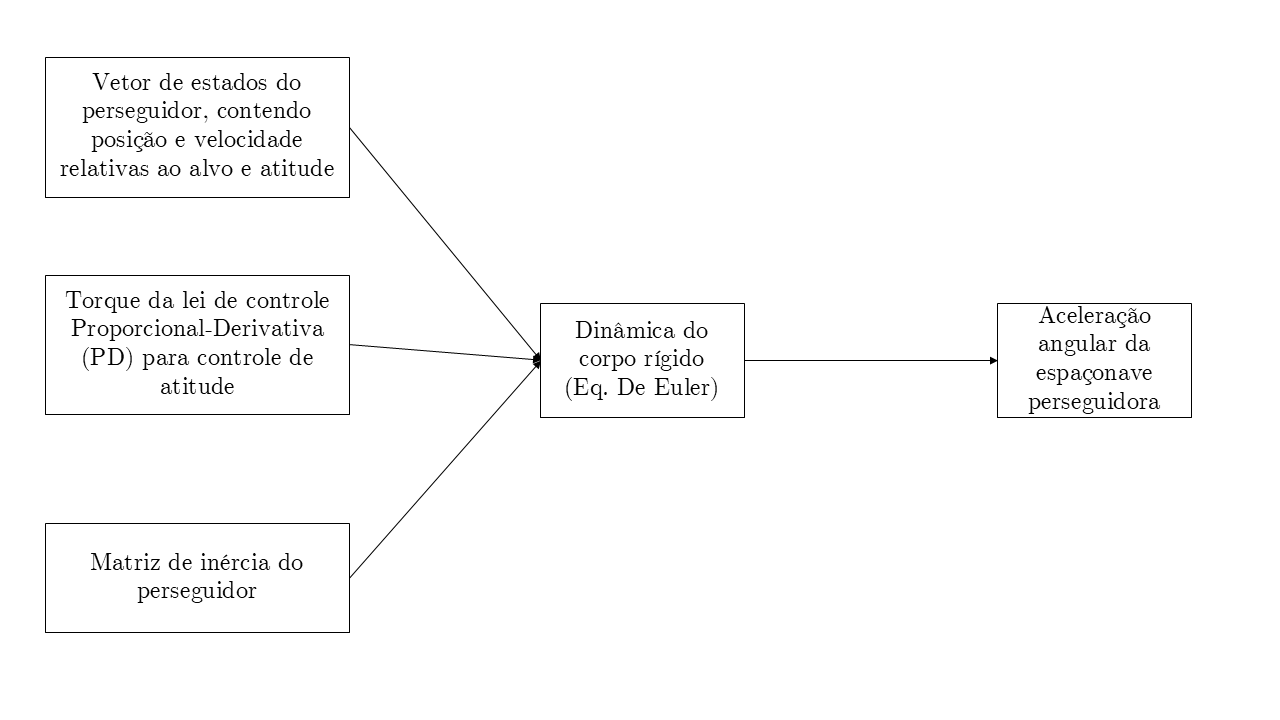
\includegraphics[width=1\linewidth]{3 Procedimento simulacao/Imagens simulink/app_final_euler_corpo_rigido.png}
\caption{Implementação das equações de Euler para a dinâmica de atitude da espaçonave no Simulink.}
\label{fig_simulink_euler}
\end{figure}

Quando o \gls{mr} inicia sua movimentação, a dinâmica do sistema passa a considerar o acoplamento entre a espaçonave e o manipulador. 
Nesse caso, utiliza-se uma formulação baseada em energia cinética e nas equações de Lagrange, permitindo representar o efeito das movimentações articulares sobre a dinâmica de atitude da espaçonave.

A Figura~\ref{fig_simulink_dinamica_acoplada} apresenta o subsistema responsável por essa modelagem. 
Nesse bloco, as variáveis generalizadas incluem tanto os estados associados à atitude da espaçonave quanto os ângulos das juntas do \gls{mr}, sendo a dinâmica governada pelas matrizes de inércia e pelos termos de Coriolis do sistema acoplado.

\begin{figure}[H]
\centering
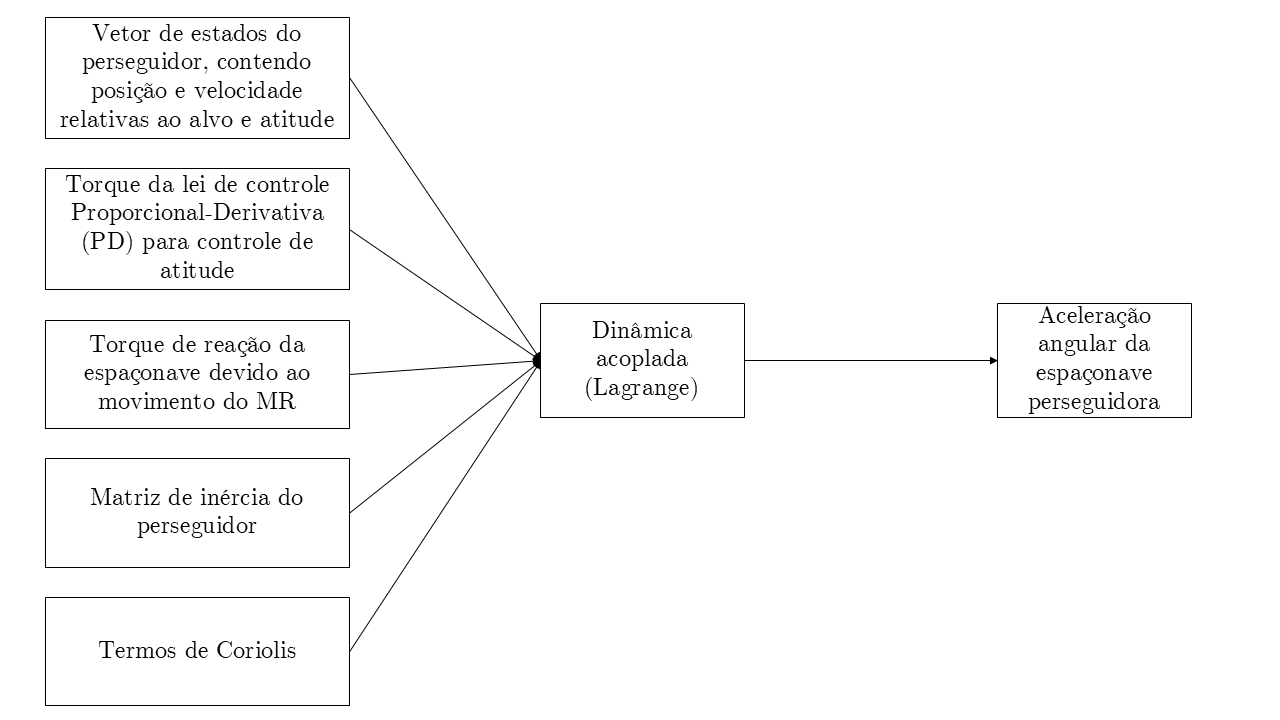
\includegraphics[width=1\linewidth]{3 Procedimento simulacao/Imagens simulink/app_final_dinamica_acoplada.png}
\caption{Implementação da dinâmica acoplada entre a espaçonave e o \gls{mr} no Simulink.}
\label{fig_simulink_dinamica_acoplada}
\end{figure}

% \begin{figure}[H]
% \centering
% 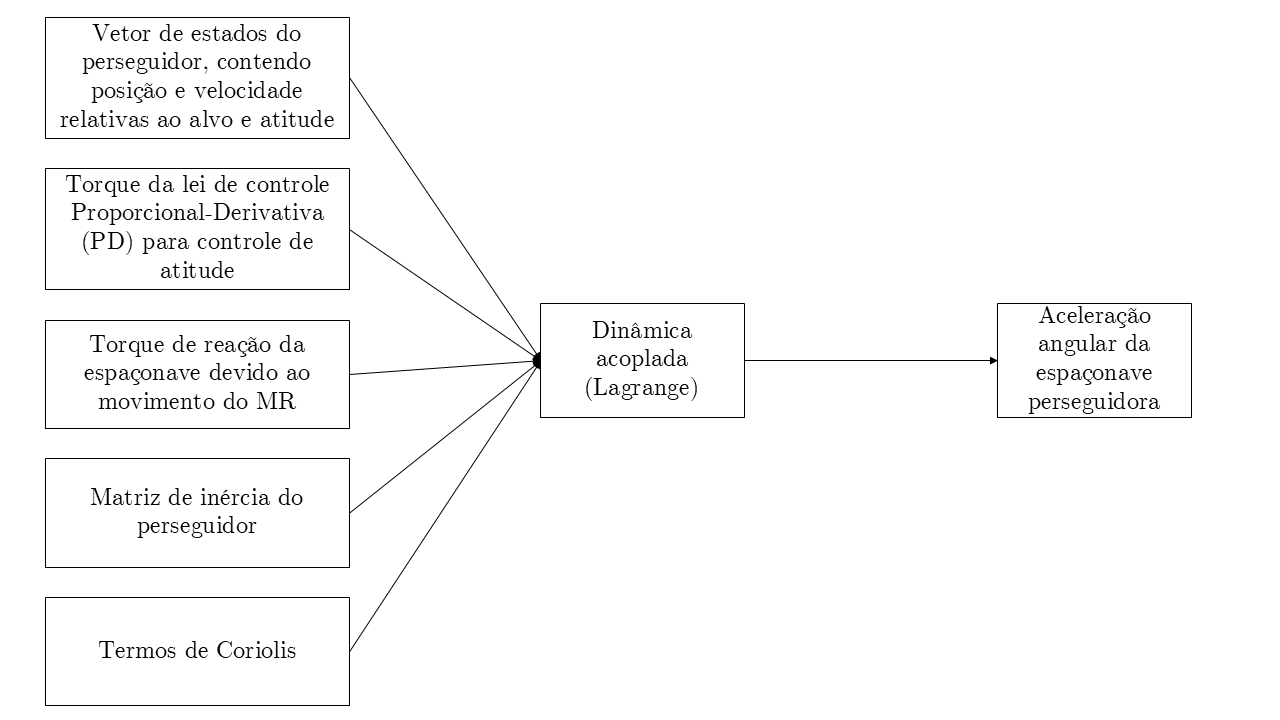
\includegraphics[angle=90,height=0.9\textheight]{3 Procedimento simulacao/Imagens simulink/app_final_dinamica_acoplada.png}
% \caption{Implementação da dinâmica acoplada entre a espaçonave e o \gls{mr} no Simulink.}
% \label{fig_simulink_dinamica_acoplada}
% \end{figure}

%%%%%%%%%%%%%%%%%%%% ALPHA TRANSICAO DINAMICAS

A transição entre o modelo de corpo rígido e o modelo dinâmico acoplado é realizada por meio de um bloco de comutação suave, conforme ilustrado na Figura~\ref{fig_simulink_transicao_dinamica}. 
Nesse bloco, foi introduzido um parâmetro de transição $\alpha$, responsável por realizar uma interpolação gradual entre as duas dinâmicas.

Essa estratégia foi adotada para evitar descontinuidades no modelo dinâmico que poderiam introduzir degraus na resposta do sistema ou causar instabilidades numéricas durante a simulação.

\begin{figure}[H]
\centering
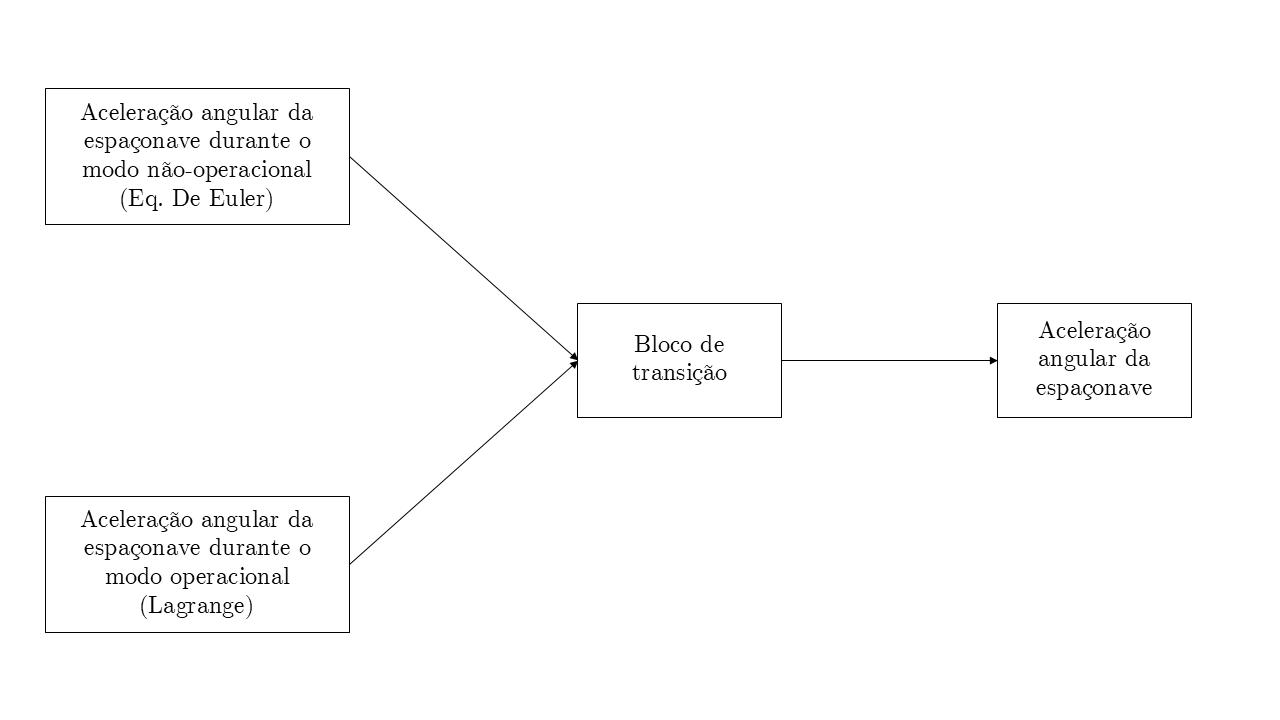
\includegraphics[width=1\linewidth]{3 Procedimento simulacao/Imagens simulink/app_final_transicao_dinamica.png}
\caption{Transição entre a dinâmica de corpo rígido e a dinâmica acoplada.}
\label{fig_simulink_transicao_dinamica}
\end{figure}

Inclusive, o mesmo $\alpha$ é utilizado para iniciar outros blocos, como a cinemática inversa e o bloco de controle \gls{pd} das juntas do \gls{mr}.
A dinâmica do sistema acoplado é governada por uma equação matricial que relaciona as variáveis generalizadas do sistema com as matrizes de inércia e os termos de Coriolis. 
O particionamento dessas matrizes, bem como sua formulação detalhada, é apresentado adiante na Equação~\ref{eq_particionamento_M_C}. 
